\documentclass[main.tex]{subfiles}
\begin{document}

% ── Block 2b: Continuous DiD (Callaway, Goodman-Bacon & Sant'Anna) ────────
% Cifras del paper: papers/CGBS2025_continuous_DiD_AER_text.md (con página).
% Cifras de la demo: R/contdid/numbers_for_slides.txt (replicación del README).
\section{Continuous Treatment: Callaway, Goodman-Bacon \& Sant'Anna}

% ── 1. Bridge from Case 3 ────────────────────────────────────────────────
\begin{frame}{From Case 3 to a Continuous Dose}

  Case 3 (East et al.'s data) gave us an effect per unit of eligibility under
  one assumption: with \texttt{continuous(1)}, that the status-quo trend is
  linear in the baseline dose. We assumed a functional form and obtained a
  scaled level.

  \medskip
  That is one route. The question underneath it is more general, and continuous
  doses are everywhere: Medicaid eligibility rates, minimum wages in euros,
  tariff schedules, pollution exposure, subsidy shares.

  \medskip
  \begin{block}{The question for this module}
    With a continuous dose, what does parallel trends identify, and what does it
    fail to identify even when it holds exactly?
  \end{block}

  \medskip
  \footnotesize Callaway, Goodman-Bacon \& Sant'Anna, \textit{Difference-in-Differences
  with a Continuous Treatment}, forthcoming \textit{AER}.

\end{frame}

% ── 2. The numbers first: reading the table by rows ──────────────────────
\begin{frame}{Did the Subsidy Work?}

  A subsidy covering a share $d$ of a firm's costs. Suppose we knew the true
  effect at every level of coverage. Illustrative numbers.

  \medskip
  \begin{columns}[T]
    \begin{column}{0.40\textwidth}
      \begin{center}\small
      \begin{tabular}{@{}lr@{}}
        \toprule
        Coverage $d$ & Effect vs no subsidy \\
        \midrule
        25\,\%  & $+2.0$ \\
        50\,\%  & $+3.5$ \\
        75\,\%  & $+4.4$ \\
        100\,\% & $+4.2$ \\
        \bottomrule
      \end{tabular}
      \end{center}
    \end{column}
    \begin{column}{0.56\textwidth}
      Each row compares one group of firms against firms that received nothing.
      Four separate comparisons, four heights above zero.

      \smallskip
      Every level of coverage beats having no subsidy, and by a wide margin. At
      full coverage the programme is worth $+4.2$.

      \smallskip
      \begin{block}{\footnotesize If the question is whether to run it}
        \footnotesize
        This table settles it. The answer is yes, at every level of coverage.
      \end{block}
    \end{column}
  \end{columns}

\end{frame}

% ── 3. The same numbers, read by steps ───────────────────────────────────
\begin{frame}{Should We Raise It?}

  Same programme, same numbers, read by steps instead of by rows.

  \medskip
  \begin{center}\small
  \begin{tabular}{@{}lrrl@{}}
    \toprule
    Step & Extra effect & Extra coverage & Per unit of coverage \\
    \midrule
    25\,\% $\to$ 50\,\%  & $+1.5$ & $0.25$ & $+1.5 / 0.25 = +6.0$ \\
    50\,\% $\to$ 75\,\%  & $+0.9$ & $0.25$ & $+0.9 / 0.25 = +3.6$ \\
    75\,\% $\to$ 100\,\% & \alert{$-0.2$} & $0.25$ & \alert{$-0.2 / 0.25 = -0.8$} \\
    \bottomrule
  \end{tabular}
  \end{center}

  \medskip
  \begin{columns}[T]
    \begin{column}{0.50\textwidth}
      The last stretch of coverage \alert{made things worse}: going from
      75\,\% to full took the effect from $+4.4$ down to $+4.2$.

      \smallskip
      The programme is worth running at every level of coverage. The last
      stretch of it is not worth paying for.
    \end{column}
    \begin{column}{0.46\textwidth}
      \begin{block}{\footnotesize Why the last column divides}
        \footnotesize
        Dividing by the step puts all three rows on the same footing: what a
        whole unit of coverage would add at that point on the curve. That is
        the number software reports, and it is why the figure changes if you
        measure the dose from $0$ to $100$ instead of from $0$ to $1$.
      \end{block}
    \end{column}
  \end{columns}

\end{frame}

% ── 4. Naming the two objects ────────────────────────────────────────────
\begin{frame}{Two Causal Objects: Height and Slope}

  The two questions have names, and they are different parameters.

  \medskip
  \begin{columns}[T]
    \begin{column}{0.46\textwidth}
      \begin{block}{Level: $ATT(d\mid d)$}
        \footnotesize
        The effect of dose $d$ against no treatment at all. The
        \emph{height} of the curve at $d$.
        \[ \mathbb{E}\!\left[Y_{t=2}(d)-Y_{t=2}(0)\mid D=d\right] \]
      \end{block}

      \smallskip
      \begin{block}{Slope: $ACRT(d\mid d)$}
        \footnotesize
        The effect of one more unit of dose. The \emph{steepness} of the curve at
        $d$.
        \[ \mathbb{E}\!\left[\left.\tfrac{\partial}{\partial l} Y_{t=2}(l)\right|_{l=d}
           \,\middle|\, D=d\right] \]
      \end{block}
    \end{column}
    \begin{column}{0.52\textwidth}
      \centering
      % f(x) = 1.5x - 0.18x^2, maximo en x = 4.17 DENTRO del dominio dibujado,
      % para que la curva llegue a girar y la pendiente se vuelva negativa
      % mientras la altura sigue muy por encima de cero.
      \begin{tikzpicture}[scale=0.80]
        \draw[->,gray] (0,0) -- (7.2,0) node[right,black,font=\scriptsize] {$d$};
        \draw[->,gray] (0,0) -- (0,4.1);
        \draw[very thick,DarkBlue] plot[domain=0:6.4,samples=80]
          (\x, {1.5*\x - 0.18*\x*\x});
        % tangente horizontal en el maximo
        \draw[thick,black!45] (3.35,3.125) -- (5.0,3.125);
        \node[font=\scriptsize,anchor=east,black!55] at (3.25,3.20) {slope $=0$};
        % dosis alta: altura positiva, pendiente negativa
        \draw[thick,MidBlue,dashed] (5.5,0) -- (5.5,2.805);
        \draw[thick,AlertRed] (4.7,3.189) -- (6.6,2.277);
        \fill[DarkBlue] (5.5,2.805) circle (2.4pt);
        \node[MidBlue,font=\scriptsize,anchor=east] at (5.3,1.30)
          {height $>0$};
        \node[AlertRed,font=\scriptsize,anchor=south] at (5.9,3.55)
          {slope $<0$};
      \end{tikzpicture}
    \end{column}
  \end{columns}

  \medskip
  A curve can be high and falling at the same time: $ATT$ stays positive at
  every dose while $ACRT$ turns negative at the top. With a binary treatment
  there is one dose and one step, so the two coincide. The figure draws a single
  curve; whose curve it is comes after the reading of the two plots.

\end{frame}

% ── 4b. How to read the two plots the command draws ──────────────────────
\begin{frame}{Reading the Two Plots}

  \begin{columns}[T]
    \begin{column}{0.44\textwidth}
      \centering
      % Panel superior ATT(d) y panel inferior ACRT(d) = su derivada,
      % alineados en d para que el maximo de arriba caiga sobre el cero
      % de abajo. f(x) = 1.5x - 0.18x^2 ; f'(x) = 1.5 - 0.36x
      \begin{tikzpicture}[scale=0.58]
        % --- panel superior: el nivel ---
        \draw[->,gray] (0,0) -- (7.3,0);
        \draw[->,gray] (0,0) -- (0,4.0)
          node[above,black,font=\scriptsize] {$ATT(d\mid d)$};
        \draw[very thick,DarkBlue] plot[domain=0:6.4,samples=80]
          (\x, {1.5*\x - 0.18*\x*\x});
        \draw[thick,black!45] (3.4,3.125) -- (4.95,3.125);
        % --- conectores verticales ---
        \draw[AlertRed,dashed,thick] (4.167,3.125) -- (4.167,-3.2);
        \draw[MidBlue,dashed] (5.9,2.63) -- (5.9,-3.83);
        % --- panel inferior: la pendiente ---
        \draw[->,gray] (0,-3.2) -- (7.3,-3.2)
          node[right,black,font=\scriptsize] {$d$};
        \draw[->,gray] (0,-4.4) -- (0,-1.3)
          node[above,black,font=\scriptsize] {$ACRT(d\mid d)$};
        \draw[very thick,MidBlue] plot[domain=0:6.4,samples=2]
          (\x, {-1.7 - 0.36*\x});
        \fill[AlertRed] (4.167,3.125) circle (2.4pt);
        \fill[AlertRed] (4.167,-3.2) circle (2.4pt);
        \node[font=\scriptsize,anchor=south,black!55] at (4.17,3.22) {flat};
        \node[font=\scriptsize,anchor=west,AlertRed] at (4.45,-2.9) {zero};
        \node[font=\scriptsize,anchor=west,MidBlue] at (6.1,2.5) {still high};
        \node[font=\scriptsize,anchor=west,MidBlue] at (6.1,-3.9) {negative};
      \end{tikzpicture}
    \end{column}
    \begin{column}{0.54\textwidth}
      The command draws both. The second is the derivative of the first,
      redrawn so that a slope becomes a height.

      \medskip
      \begin{itemize}
        \item The \textbf{height} of the top plot at $d$ is the level,
          $ATT(d\mid d)$.
        \item The \textbf{slope} of the top plot at $d$ is the
          \textbf{height} of the bottom plot at $d$.
        \item Where the top curve flattens, the bottom one
          \alert{crosses zero}.
        \item Where the top curve turns down, the bottom one is
          \alert{negative}, and the level up there is still well above zero.
      \end{itemize}

    \end{column}
  \end{columns}

  \smallskip
  \footnotesize \textbf{Why draw the second at all:} you cannot put a confidence
  band on ``that curve looks steep''. Turning the slope into a height gives it a
  standard error.

\end{frame}

% ── 4c. One observed point per dose group ────────────────────────────────
\begin{frame}{One Point per Dose Group}

  \begin{columns}[T]
    \begin{column}{0.56\textwidth}
      \centering
      % Tres curvas de grupo (misma forma, distinta altura), un punto negro
      % por grupo en su propia dosis, dos huecos en d2 sobre las otras curvas,
      % y la curva roja que une los puntos (cuadratica por los tres puntos).
      \begin{tikzpicture}[scale=0.66]
        \draw[->,gray] (0,0) -- (7.0,0) node[right,black,font=\scriptsize] {dose $l$};
        \draw[->,gray] (0,0) -- (0,5.3) node[above,black,font=\scriptsize] {effect};
        \draw[thick,DarkBlue!55] plot[domain=0.6:6.3,samples=60] (\x, {1.2*\x - 0.12*\x*\x});
        \draw[thick,DarkBlue!75] plot[domain=0.6:6.3,samples=60] (\x, {0.7 + 1.2*\x - 0.12*\x*\x});
        \draw[thick,DarkBlue] plot[domain=0.6:6.3,samples=60] (\x, {1.4 + 1.2*\x - 0.12*\x*\x});
        \node[DarkBlue!55,font=\scriptsize,anchor=west] at (6.35,2.80) {group $d_1$};
        \node[DarkBlue!75,font=\scriptsize,anchor=west] at (6.35,3.50) {group $d_2$};
        \node[DarkBlue,font=\scriptsize,anchor=west] at (6.35,4.20) {group $d_3$};
        \draw[very thick,AlertRed,dashed] plot[domain=1.0:5.6,samples=60] (\x, {-0.646 + 1.64*\x - 0.126*\x*\x});
        \node[AlertRed,font=\scriptsize,anchor=south west,align=left] at (0.5,4.45) {joins the observed points:\\ $d \mapsto ATT(d\mid d)$};
        \fill[black] (1.5,1.53) circle (2.6pt); \fill[black] (3.2,3.31) circle (2.6pt); \fill[black] (5.0,4.40) circle (2.6pt);
        \draw[gray,dashed] (1.5,0) -- (1.5,1.53); \draw[gray,dashed] (3.2,0) -- (3.2,3.31); \draw[gray,dashed] (5.0,0) -- (5.0,4.40);
        \node[font=\scriptsize,below] at (1.5,0) {$d_1$}; \node[font=\scriptsize,below] at (3.2,0) {$d_2$}; \node[font=\scriptsize,below] at (5.0,0) {$d_3$};
        \draw[DarkBlue!55,thick] (3.2,2.61) circle (2.4pt); \draw[DarkBlue,thick] (3.2,4.01) circle (2.4pt);
        \node[font=\scriptsize,anchor=north west,black!70,align=left] at (3.45,2.05) {hollow: what $d_2$ would\\ have done to the others};
      \end{tikzpicture}
    \end{column}
    \begin{column}{0.42\textwidth}
      \footnotesize
      \begin{itemize}
        \item Each dose group has its own response curve: what every dose $l$
          would have done to it. Groups can respond by different amounts.
        \item The data show \textbf{one point per group}: the group at $d_2$
          is observed at $d_2$ and nowhere else.
        \item \textbf{Local}, $ATT(d\mid d)$: the black dot of group $d$.
          $ATT^{\text{loc}}$ averages the dots.
        \item \textbf{Global}, $ATT(d)$: the effect of dose $d$ on all treated
          groups. At $d_2$, the vertical average of the black dot and the two
          hollow ones, which are never observed.
      \end{itemize}
    \end{column}
  \end{columns}

  \smallskip
  \begin{alertblock}{\footnotesize The red curve}
    \footnotesize
    It joins the black dots and is the only curve the data can draw. It is not
    the curve of any group: each point comes from a different group. Here it is
    steeper than every group's curve, because higher-dose groups respond more at
    every dose.
  \end{alertblock}

\end{frame}

% ── 5. What parallel trends identifies ───────────────────────────────────
\begin{frame}{What Parallel Trends Identifies}

  \begin{block}{What you can identify: the height of the curve}
    Under parallel trends, for every dose $d$ in the support (Theorem 3.1, p.~10):
    \[
      ATT(d\mid d) \;=\; \mathbb{E}\!\left[\Delta Y \mid D=d\right]
        - \mathbb{E}\!\left[\Delta Y \mid D=0\right],
    \]
    \[
      ATT^{\text{loc}} \;=\; \mathbb{E}\!\left[\Delta Y \mid D>0\right]
        - \mathbb{E}\!\left[\Delta Y \mid D=0\right].
    \]
  \end{block}

  \medskip
  One DiD per dose, each against the untreated. Nothing exotic: it is the
  comparison of means you already know, run separately at every value of $d$.

  \medskip
  \begin{itemize}
    \item The whole curve $d \mapsto ATT(d\mid d)$ is identified.
    \item $ATT^{\text{loc}}$ averages it over the treated, and equals a plain
      binary DiD on $\mathbf{1}\{D>0\}$.
    \item Every comparison here is anchored on the untreated group.
  \end{itemize}

  \medskip
  In the picture: parallel trends pins the height of every black dot, and joined
  they trace the red curve. It does not justify comparing two dots with each
  other.

\end{frame}

% ── 6. Differentiating the joined curve compares two groups ──────────────
\begin{frame}{Differentiating the Joined Curve Compares Two Groups}

  \begin{columns}[T]
    \begin{column}{0.50\textwidth}
      \centering
      % Figura 3 del paper: dos curvas de grupo, un punto negro en cada una,
      % la cuerda roja entre los puntos, el hueco y el salto en d.
      \begin{tikzpicture}[scale=0.68]
        \draw[->,gray] (0,0) -- (7.0,0) node[right,black,font=\scriptsize] {dose $l$};
        \draw[->,gray] (0,0) -- (0,4.4);
        \draw[very thick,DarkBlue] plot[domain=0.5:6.2,samples=60] (\x, {1.2*\x - 0.12*\x*\x});
        \draw[very thick,MidBlue] plot[domain=0.5:6.2,samples=60] (\x, {1.2*\x - 0.12*\x*\x + 0.9});
        \node[DarkBlue,font=\scriptsize,anchor=west] at (6.25,2.98) {group $d$};
        \node[MidBlue,font=\scriptsize,anchor=west] at (6.25,3.9) {group $d'$};
        \fill[black] (2.5,2.25) circle (2.4pt);
        \fill[black] (4.0,3.78) circle (2.4pt);
        \draw[MidBlue,thick] (2.5,3.15) circle (2.2pt);
        \draw[AlertRed,thick] (2.5,2.25) -- (4.0,3.78);
        \draw[MidBlue,dashed] (2.5,3.15) -- (4.0,3.78);
        \draw[gray,dashed] (2.5,0) -- (2.5,2.25); \draw[gray,dashed] (4.0,0) -- (4.0,3.78);
        \node[font=\scriptsize,below] at (2.5,0) {$d$}; \node[font=\scriptsize,below] at (4.0,0) {$d'$};
        \node[AlertRed,font=\scriptsize,anchor=north west,fill=white,inner sep=1pt] at (3.1,2.55) {what is measured};
        \node[MidBlue,font=\scriptsize,anchor=south east] at (3.9,3.95) {own slope};
        \draw[<->,black!60] (2.35,2.25) -- (2.35,3.15);
        \node[font=\scriptsize,anchor=east,black!60,fill=white,inner sep=1pt] at (2.3,2.7) {jump};
      \end{tikzpicture}
    \end{column}
    \begin{column}{0.48\textwidth}
      \footnotesize
      Two black dots, one per group. The red chord between them is what a
      difference, or a derivative, measures, and it adds two pieces
      (Theorem 3.2, p.~11); divided by $d'-d$, the first is $ACRT(d'\mid d')$:
      \[
        \underbrace{\vphantom{\big(}\text{own step of group } d'}_{ATT(d'\mid d') - ATT(d\mid d')}
        \;+\;
        \underbrace{\text{jump between curves at } d}_{ATT(d\mid d') - ATT(d\mid d)}
      \]
      \begin{itemize}
        \item The jump runs up to the hollow dot, what dose $d$ would have
          done to group $d'$. Never observed, so \textbf{not identified}.
        \item Parallel trends says nothing about it. The paper calls it a
          version of \textbf{selection on gains} (p.~11).
        \item An infinitesimal step changes nothing: $d$ against
          $d+\varepsilon$ is still two groups.
      \end{itemize}
    \end{column}
  \end{columns}

  \smallskip
  \footnotesize In the continuous limit:
  $\dfrac{\partial\, \mathbb{E}[\Delta Y\mid D=d]}{\partial d}
   = ACRT(d\mid d) + \left.\dfrac{\partial\, ATT(d\mid l)}{\partial l}\right|_{l=d}$.

\end{frame}

% ── 6b. Same slopes, still biased ────────────────────────────────────────
\begin{frame}{Same Slopes, Still Biased}

  Two firms with the \emph{same slope} from 25\,\% to 50\,\%: A receives
  25\,\% coverage, B receives 50\,\%.

  \medskip
  \begin{center}\small
  \begin{tabular}{@{}lcc@{}}
    \toprule
     & Effect if coverage 25\,\% & Effect if coverage 50\,\% \\
    \midrule
    Firm A (receives 25\,\%) & $\mathbf{2.0}$ (observed) & $3.0$ \\
    Firm B (receives 50\,\%) & $3.0$ & $\mathbf{4.0}$ (observed) \\
    \bottomrule
  \end{tabular}
  \end{center}

  \medskip
  \begin{columns}[T]
    \begin{column}{0.48\textwidth}
      \begin{block}{\footnotesize What is measured}
        \footnotesize
        $4.0 - 2.0 = 2.0$. The causal response of going from 25\,\% to
        50\,\% is $1.0$ on both curves. The other $1.0$ is that B responds
        one unit more than A at 25\,\% coverage.
      \end{block}
    \end{column}
    \begin{column}{0.48\textwidth}
      \begin{block}{\footnotesize What this says}
        \footnotesize
        The jump is the gap between the curves at the lower dose: $3.0 - 2.0$
        at 25\,\%. Both curves start at zero effect at zero coverage, so that
        gap is the slope difference below 25\,\% (B rises $3.0$, A rises
        $2.0$). Equal slopes from 25\,\% to 50\,\% do not remove it.
      \end{block}
    \end{column}
  \end{columns}

  \medskip
  \footnotesize Selection on gains: groups with different doses would gain
  different amounts from the \emph{same} dose (here B gains more; in other data
  the gap goes the other way). Units may choose their dose for that reason, or
  exposure may go with responsiveness (for exposure doses the paper suggests
  ``heterogeneity bias'', fn.~2).

\end{frame}

% ── 7. Strong parallel trends and the untestable difference ──────────────
\begin{frame}{Strong Parallel Trends, and Why No Pre-Test Finds It}

  Strong parallel trends: at every dose $d$, all treated units, had they
  received $d$, would have followed the path dose group $d$ actually followed
  (p.~12). With PT, \textbf{each black dot equals the average of the dots at
  its dose}; all groups sharing one curve is the simplest case.

  \medskip
  \begin{columns}[T]
    \begin{column}{0.50\textwidth}
      \begin{block}{\footnotesize What follows (Theorem 3.3, p.~13)}
        \footnotesize
        The joined red curve is then the global curve $ATT(d)$, the average
        over all treated. Its derivative is the $ACRT$, its maximum is the dose
        past which more adds nothing. With PT, $ATT(d) = ATT(d\mid d)$.
        \[
          ACRT(d) \;=\; \frac{\partial\, \mathbb{E}[\Delta Y \mid D=d]}{\partial d}.
        \]
      \end{block}
    \end{column}
    \begin{column}{0.48\textwidth}
      \begin{alertblock}{\footnotesize The paper, p.~13}
        \footnotesize
        ``Strong parallel trends only changes the interpretation of the
        estimand, not its form.''
      \end{alertblock}
      \smallskip
      \footnotesize The formula under PT and under SPT is \textbf{the same
      formula}: estimate the red curve and differentiate. What changes is
      whether the result may be called a causal response.
    \end{column}
  \end{columns}

  \medskip
  \footnotesize A pre-period only shows untreated potential outcomes, so no
  event-study plot, placebo or joint test can tell the two assumptions apart.
  The authors (p.~3): it is common for papers to write as if they had assumed
  the weak version and interpret as if they had assumed the strong one.

\end{frame}

% ── 7b. The four summaries and the two labels ───────────────────────────
\begin{frame}{Four Summaries, Two Labels}
  \begin{center}\footnotesize
  \begin{tabular}{@{}p{3.6cm}p{4.6cm}p{4.6cm}@{}}
    \toprule
    & Level & Slope \\
    \midrule
    \textbf{Local}: each group at its own dose
      & $ATT^{\text{loc}} = \mathbb{E}[ATT(D\mid D)\mid D>0]$, the average of the black dots
      & $ACRT^{\text{loc}} = \mathbb{E}[ACRT(D\mid D)\mid D>0]$, the average own-curve slope \\[3pt]
    \textbf{Global}: one dose for every treated group
      & $ATT^{\text{glob}} = \mathbb{E}[ATT(D)\mid D>0]$, hollow dots included
      & $ACRT^{\text{glob}} = \mathbb{E}[ACRT(D)\mid D>0]$ \\
    \bottomrule
  \end{tabular}
  \end{center}
  \smallskip
  \footnotesize
  Firms: $ATT^{\text{loc}} = (2.0 + 4.0)/2 = 3.0$ needs only what is observed;
  $ATT(25\,\%) = (2.0 + 3.0)/2 = 2.5$ needs B's unobserved $3.0$.
  \medskip
  \begin{columns}[T]
    \begin{column}{0.48\textwidth}
      \begin{block}{\footnotesize Parallel trends identifies one cell}
        \footnotesize
        The local level: $ATT^{\text{loc}}$ is the binary DiD on
        $\mathbf{1}\{D>0\}$. The global level needs the hollow dots. No slope
        exists with one point per curve, not even the local one.
      \end{block}
    \end{column}
    \begin{column}{0.48\textwidth}
      \begin{block}{\footnotesize Strong parallel trends fills the global row}
        \footnotesize
        With PT, $ATT(d\mid d) = ATT(d)$: local $=$ global for the level. The
        joined curve's derivative is the global $ACRT(d)$, not $ACRT(d\mid d)$.
      \end{block}
    \end{column}
  \end{columns}
  \medskip
  \footnotesize \textbf{Which assumption gives which summary.} PT identifies
  the local level $ATT^{\text{loc}}$ (Thm 3.1); with SPT the same number is also
  global. The slope needs SPT, and the paper's SPT, which holds on average over
  dose groups, gives the global $ACRT^{\text{glob}}$ (Cor.~3.1).
  $ACRT^{\text{loc}}$ needs SPT for every dose group (App.~C, fn.~13).
\end{frame}
% ── 10. Software ─────────────────────────────────────────────────────────
\begin{frame}[fragile]{Software: the \texttt{contdid} Package}

\lstset{
  language={},
  basicstyle=\scriptsize\ttfamily,
  keywordstyle=\color{MidBlue},
  commentstyle=\color{gray},
  breaklines=true,
  showstringspaces=false
}

\begin{lstlisting}
install.packages("contdid")   # R, CRAN 0.1.1
cont_did(yname = "Y", tname = "time_period", idname = "id", dname = "D",
         gname = "G", data = df,
         target_parameter = "slope",      # "level" for ATT(d|d)
         aggregation = "dose",            # or "eventstudy"
         control_group = "notyettreated",
         num_knots = 1, degree = 3, biters = 100, cband = TRUE)
\end{lstlisting}

  \medskip
  \begin{columns}[T]
    \begin{column}{0.48\textwidth}
      \begin{block}{\footnotesize The dose variable}
        \footnotesize
        It must be time-invariant, and it must carry its actual value in the
        pre-treatment periods. Do not code it as zero before treatment.
      \end{block}
    \end{column}
    \begin{column}{0.48\textwidth}
      \begin{alertblock}{\footnotesize Not yet supported, per the authors}
        \footnotesize
        Discrete treatments, repeated cross-sections, unbalanced panels,
        time-varying doses, covariates. The data-driven dose model
        (\texttt{cck}) needs exactly two periods, so no staggered adoption.
      \end{alertblock}
    \end{column}
  \end{columns}

  \medskip
  \footnotesize The README calls it an alpha version and says the API may
  change.

\end{frame}

% ── 12. Demo 2: un panel de hospitales con joroba ────────────────────────
\begin{frame}{Demo (2): A Hospital Panel With a Real Dose}

  \begin{columns}[T]
    \begin{column}{0.52\textwidth}
      \textbf{The reform.} Medicare's Prospective Payment System, 1983--84.
      Medicare had reimbursed a share of labor and capital costs; PPS replaced
      only the labor part, with a fixed fee per diagnosis, so capital became
      cheaper relative to labor.

      \smallskip
      \textbf{Why a dose and not a switch.} The reform is identical for every
      hospital. What differs is \textbf{exposure}: a hospital with 60\,\% of its
      patients on Medicare feels it far more than one with 10\,\%.

      \smallskip
      \textbf{The dose.} Medicare share of inpatient days in 1983; zero for
      hospitals with no Medicare patients (in the paper's data, children's and
      psychiatric).

      \smallskip
      \textbf{The outcome.} Depreciation share of costs, a proxy for capital
      intensity.
    \end{column}
    \begin{column}{0.44\textwidth}
      \begin{block}{\footnotesize The panel}
        \footnotesize
        6{,}000 hospitals, 1980--1986. \textbf{29\,\%} have zero exposure and
        act as the comparison group; the rest are spread over
        $[0.05,\,0.89]$. The reform lands in 1984.

        \smallskip
        Pre- and post-periods are averaged into two, following the paper's own
        application (1980--83 against 1984--86, p.~25).
      \end{block}

      \smallskip
      \begin{alertblock}{\footnotesize These data are simulated}
        \footnotesize
        The real AHA hospital survey must be bought from the association, so
        nobody can ship it. This is a third party's simulation of that panel,
        published in another paper's replication package. \textbf{It is not a
        replication of Acemoglu \& Finkelstein, nor of the paper's application.}
        Its virtue is that the effect was imposed, so we know the answer.
      \end{alertblock}
    \end{column}
  \end{columns}

\end{frame}

% ── 12b. El resultado sobre esos datos ───────────────────────────────────
\begin{frame}{Demo (2): Level and Slope Estimates}

  \begin{columns}[T]
    \begin{column}{0.5\textwidth}
      \centering
      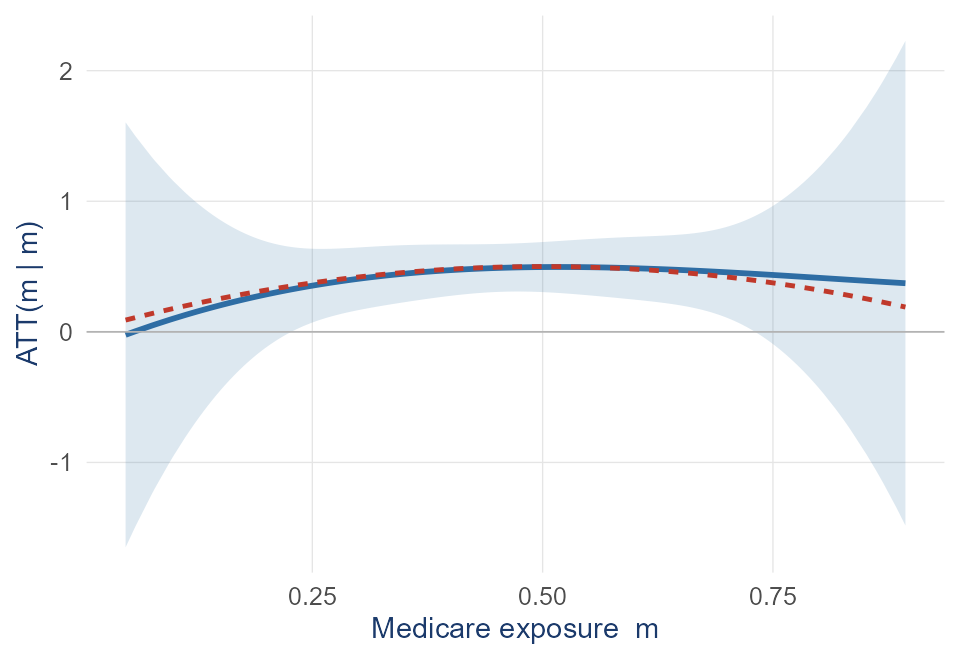
\includegraphics[width=\linewidth]{figures/contdid/fig06_af_att.png}
    \end{column}
    \begin{column}{0.5\textwidth}
      \centering
      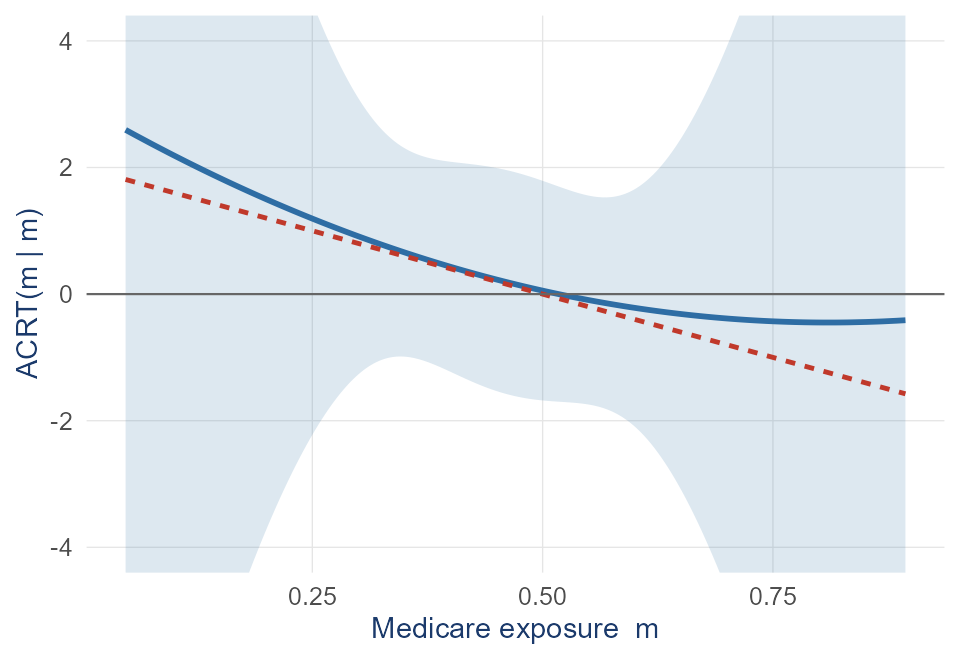
\includegraphics[width=\linewidth]{figures/contdid/fig07_af_acrt.png}
    \end{column}
  \end{columns}

  \smallskip
  \begin{columns}[T]
    \begin{column}{0.46\textwidth}
      \footnotesize
      \begin{tabular}{@{}lrr@{}}
        \toprule
        & Estimated & True \\
        \midrule
        $ATT^{\text{loc}}$   & $0.4526$ & $0.4548$ \\
        $ACRT^{\text{glob}}$ & $0.3118$ & $0.1713$ \\
        Slope crosses zero at & $m=0.517$ & $m=0.500$ \\
        \bottomrule
      \end{tabular}

    \end{column}
    \begin{column}{0.50\textwidth}
      \footnotesize
      Blue is the estimated curve, the joined dots of the theory, with its
      band; red dashed is the truth built into the simulation, one curve for
      every hospital. The true level is positive at every exposure. The slope
      changes sign near the middle, and past that point \alert{more exposure
      made things worse}, where \textbf{38\,\%} of hospitals sit.
    \end{column}
  \end{columns}

  % cifras y figuras: R/contdid/03_af_simulated.R
  \scriptsize The slope summary is $0.68$ SE from the truth. It looks further
  because $ACRT$ runs from $+1.8$ to $-1.6$ here, so the average cancels.

\end{frame}

% ── 14. dCH continuous() vs CGBS ─────────────────────────────────────────
\begin{frame}{dCH \texttt{continuous()} and CGBS Compared}

  \begin{center}\footnotesize
  \begin{tabular}{@{}p{0.20\textwidth}p{0.36\textwidth}p{0.36\textwidth}@{}}
    \toprule
    & dCH \texttt{continuous(K)} & CGBS \\
    \midrule
    Assumption & status-quo trend is a degree-$K$ polynomial in the baseline dose
      & parallel trends for the level, strong parallel trends for the slope \\[2pt]
    Identifies & the level effect of the switch by default; \textbf{per unit
      of dose} with \texttt{normalized} and in \texttt{Av\_tot\_eff}, a
      scaled level, not a derivative
      & $ATT(d\mid d)$ under PT, the global $ACRT(d)$ only under SPT \\[2pt]
    Control group & stayers, after netting out the modelled trend
      & the untreated, dose by dose \\[2pt]
    Non-absorbing & yes & no \\[2pt]
    Inference & bootstrap recommended & multiplier; opt-in uniform bands \\[2pt]
    Software & Stata, mature & R, alpha \\
    \bottomrule
  \end{tabular}
  \end{center}

  \smallskip
  \begin{block}{\footnotesize The verdict of the JEL practitioners' guide (Baker et al.\ 2025, p.~61)}
    \footnotesize
    ``These papers target different causal parameters, put more emphasis on
    different DiD designs, and, therefore, should be viewed as \textbf{complements
    rather than substitutes}.''
  \end{block}

  \smallskip
  \footnotesize dCH agree in print: their own survey lists CGBS as an estimator
  for the continuous-and-staggered design (2023, \textit{Econometrics Journal},
  Table~2, p.~C27). If your treatment switches on and off, dCH is the one that
  applies. If it is absorbing and the shape of the dose response is the question,
  CGBS is.

\end{frame}

\end{document}
